\chapter{Setting up the Workspace for C Projects}
 
Before you can start with C, some preconditions must be fulfilled:

\begin{description}
\item{A C compiler} must be installed on your machine (all tests and tutorials are based on MinGW)
\item{The CDT-Eclipse plugin} must be installed as the C development environment.
\end{description}

Once the CDT is installed, the C runtime and model library must be imported. 
(\textit{File->New->Project->eTrice} select \textit{eTrice C runtime} / \textit{eTrice C modellib})

The resulting workspace should look like this:

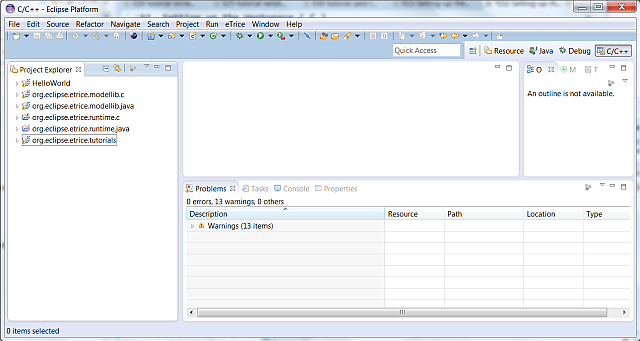
\includegraphics{images/032-SetupWorkspaceC01.png}
% !images/032-SetupWorkspaceC01.png!


\section{Testing the environment}

To verify the C tool chain you should generate and run the Hello World example program of the CDT. 
Activate the \textit{C/C++} perspective. 

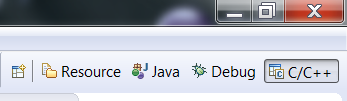
\includegraphics{images/032-SetupWorkspaceC03.png} 
% !images/032-SetupWorkspaceC03.png!
 
From the main menu select \textit{File->New->C Project}.
 
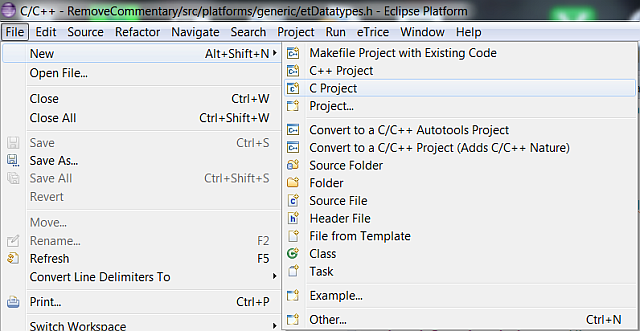
\includegraphics{images/032-SetupWorkspaceC02.png}
% !images/032-SetupWorkspaceC02.png!

Name the project. Select an \textit{Executable->Hello World ANSI C} as project type, \textit{MinGW GCC} as 
tool chain and click \textit{Finish}. 
 
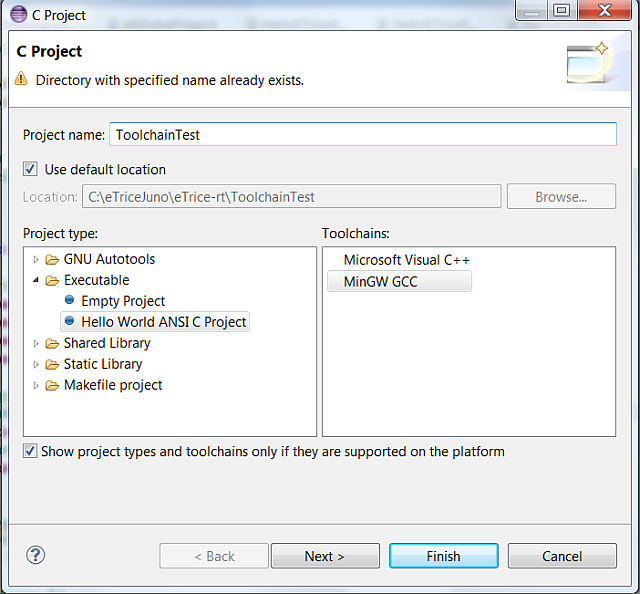
\includegraphics{images/032-SetupWorkspaceC04.png}
% !images/032-SetupWorkspaceC04.png! 

Select the new project and click the build button (or right click the project and select \textit{Build 
Project})

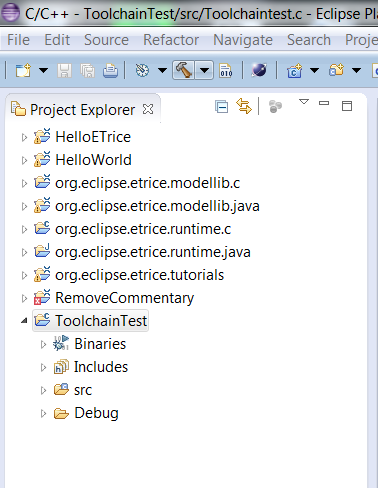
\includegraphics{images/032-SetupWorkspaceC05.png}
% !images/032-SetupWorkspaceC05.png!

The binary should be generated. Run the binary as \textit{Local C/C++ Application}.

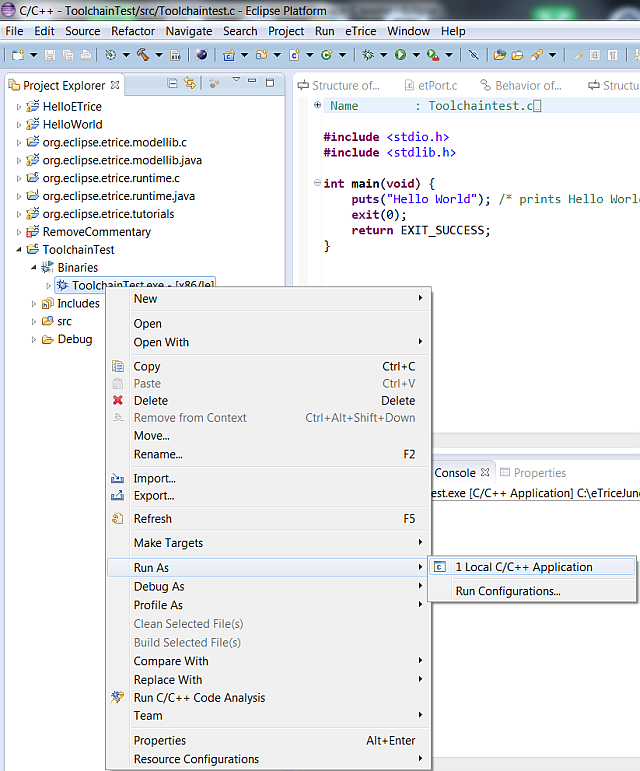
\includegraphics{images/032-SetupWorkspaceC06.png}
% !images/032-SetupWorkspaceC06.png!

Verify the output.

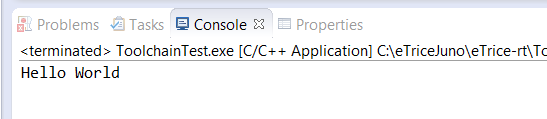
\includegraphics{images/032-SetupWorkspaceC07.png}
% !images/032-SetupWorkspaceC07.png!

Remember these steps. In the following Tutorials these steps will be referenced as \textit{build and run}.


\section{Building the C runtime system}

The C runtime system contains some basic functionalities to run the generated models. The so called 
runtime is common for all C projects. The requirements for several projects may differ depending on the 
functionality of the model or the resources of the different platforms. Therefore the runtime is 
configurable in terms of message queue size, frequency and memory alignment. The configuration file 
\textit{etRuntimeConfig.h} is located in \textit{src/config}.

After changing the configuration, the runtime must be built.

Open the properties of the \textit{org.eclipse.runtime.c} project and select \textit{C/C++ 
Build->Settings->Tool Settings} and select \textit{Includes}.

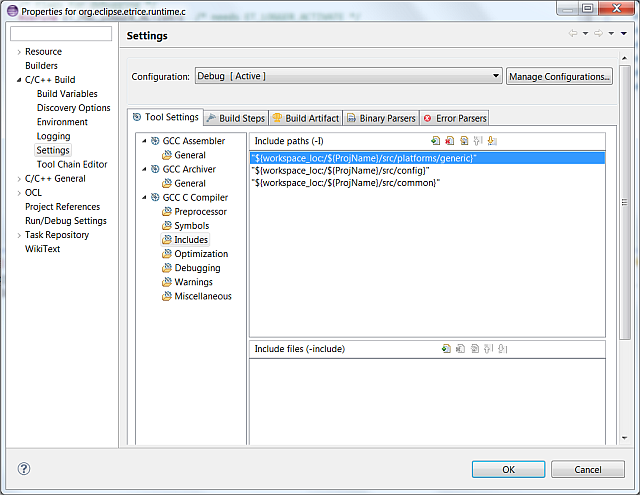
\includegraphics{images/032-SetupWorkspaceC08.png}
% !images/032-SetupWorkspaceC08.png!

Verify the include paths

\begin{itemize}
\item \textit{src/config}
\item \textit{src/common}
\item \textit{src/platforms/generic}
\end{itemize}

Within the Setting dialog select the tab \textit{Build Artefact} and select \textit{Static Library}

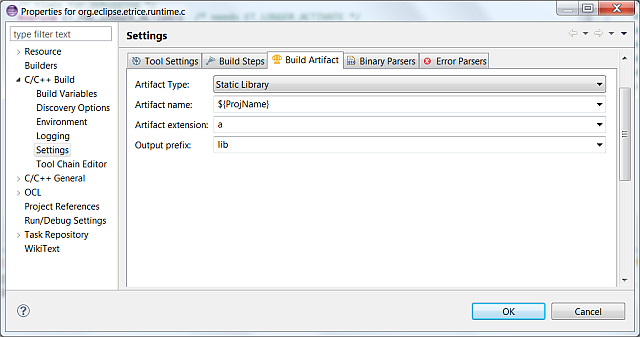
\includegraphics{images/032-SetupWorkspaceC09.png}
% !images/032-SetupWorkspaceC09.png!

Build the runtime by clicking

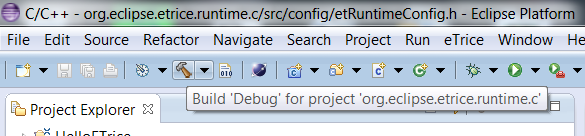
\includegraphics{images/032-SetupWorkspaceC10.png}
% !images/032-SetupWorkspaceC10.png!

The runtime library should be created.

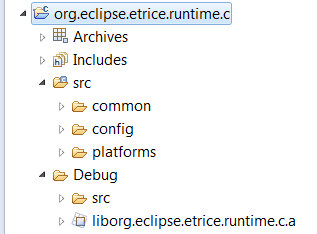
\includegraphics{images/032-SetupWorkspaceC11.png}
% !images/032-SetupWorkspaceC11.png!

For the tutorials one runtime library should be sufficient. For embedded projects it might be necessary to 
build project specific runtime libraries. In this case a separate project for the runtime should be 
created. Symbolic links to the sources might be used to avoid duplicate files. Just the configuration file 
must be duplicated. A specific library file must exist within the project. Such specific runtime libraries 
might be referenced from several applications.     
